\chapter{Metodologia}

\section{Considerações Iniciais}

Este capítulo visa apresentar a estrutura laboratorial concebida com fins de atingir os requisitos experimentais estabelecidos para validação da unidade eólica.
Os objetivos principais são:
\begin{itemize}
	\item Descrição do arranjo laboratorial;
	\item Descrição das etapas de simulação computacional e experimental para validação da bancada.
\end{itemize}

\section{Estrutura Laboratorial}

A Fig. \ref{fig:bancada-eolica} apresenta a estrutura utilizada no protótipo. Esta estrutura é levemente similar a estruturas eólicas comerciais e oferecerá recursos para análise de sistemas eólicos mais complexos.

\begin{figure}[!hbt]
	\begin{center}
    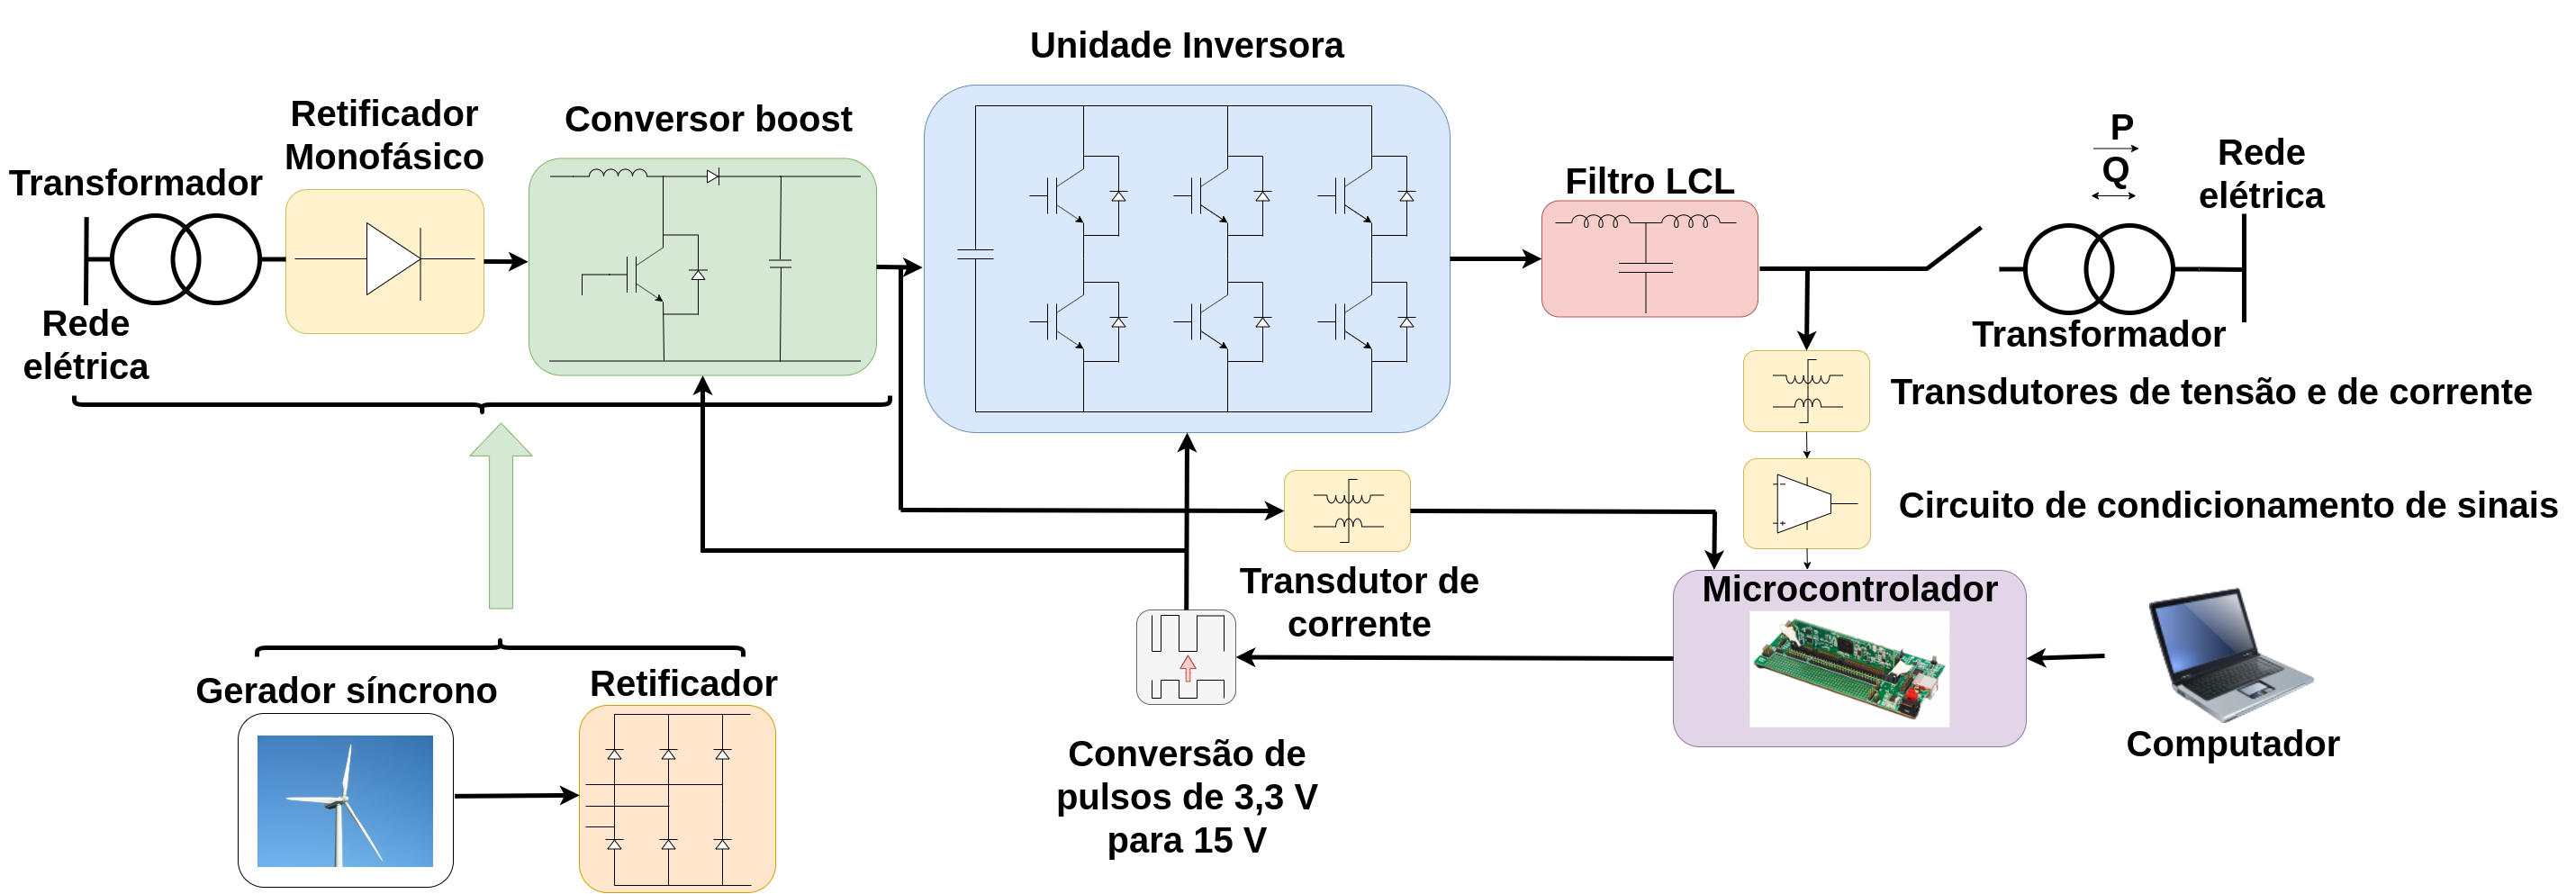
\includegraphics[scale=0.16]{figuras/Estrutura_Laboratorial.png}
    \caption{Composição da Bancada Eólica}
    \label{fig:bancada-eolica}
    \end{center}
\end{figure}

Conforme pode-se visualizar na Fig. \ref{fig:bancada-eolica}, o protótipo é constituído pela unidade de potência e unidade de controle. 

A unidade de potência é composta  pelo inversor trifásico, o filtro de acomplamento, o conversor \textit{boost}, o retificador monofásico e a própria rede elétrica. 
O conversor \textit{boost}, junto com retificador e a rede elétrica, simulam o fornecimento de potência ativa pela turbina eólica através do retificador trifásico.
A unidade de potência tem como objetivo principal a transferência de potência ativa entre o gerador síncrono, que seria a turbina éolica, e a rede elétrica.

A unidade de controle é composta pelos transdutores de tensão e de corrente, placas de condicionamento de sinais, microcontrolador, computador e adaptadores de tensão. 
O objetivo principal da unidade de controle é o monitoramento de tensões e correntes no ponto de conexão do inversor com a rede elétrica de forma a fornecer as entradas para as iterações do algoritmo de controle.

\section{Unidade de Potência}

\subsection{Conjunto Inversor Trifásico}

O inversor utilizado denomina-se SPCIT 1000-80-20. Esta, em conjunto com a unidade de controle, compõem a unidade inversora proposta, como pode ser visualizado na Fig. \ref{fig:conjunto-inversor}.
Suas principais características são:

\begin{figure}[!hbt]
	\begin{center}
    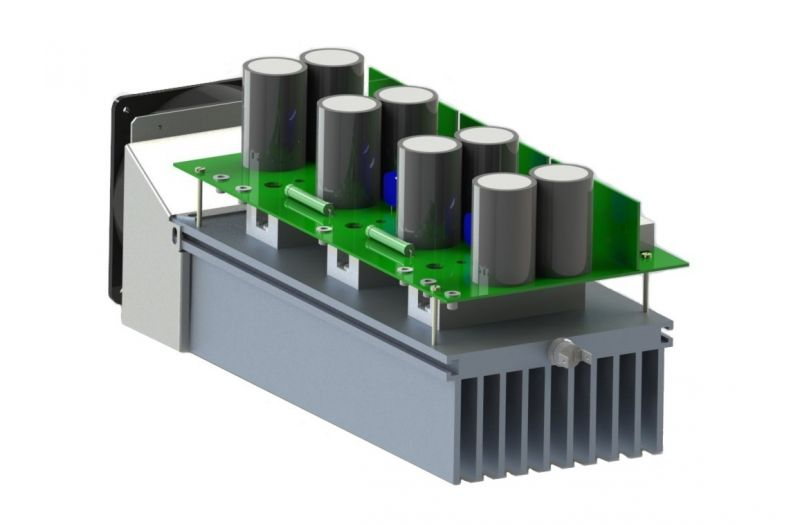
\includegraphics[scale=0.3]{figuras/conjunto_inversor_trifasico.jpg}
    \caption{Conjunto Inversor Trifásico SPCIT 1000-80-20. Fonte: Supplier}
    \label{fig:conjunto-inversor}
    \end{center}
\end{figure}

\begin{itemize}
	\item Inversor trifásico de três braços na topologia meia-ponte;
	\item Braços compostos por IGBTs do tipo LUH100G1201, conforme a Fig. \ref{fig:igbt-LUH100G1201}, equipado com \textit{gate drivers} DRO100D25A, conforme a Fig. \ref{fig:driver-DRO100D25A}.
	\item Tensão máxima de barramento: 800 $V_{CC}$ + 10 \%;
	\item Frequência máxima de chaveamento: 20 kHz;
	\item Potência Nominal: 10 kVA:
	\item Tensão de saída: 0 - 380 $V_{RMS(F-F)}$;
	\item Frequência de saída: 30 - 150 Hz;
	\item Corrente máxima de saída: 15,2 A para 380 $V_{F-F}$, tensão de barramento em 800 V, frequência de chaveamento 10 kHz;
	\item Ventilador ASA 12038DV-HB e termostato para proteção térmica.
	
\end{itemize}

\begin{figure}[!hbt]
	\begin{center}
    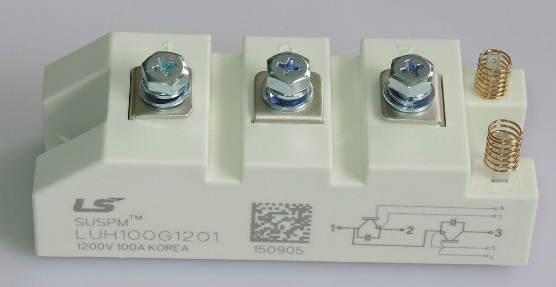
\includegraphics[scale=0.3]{figuras/LUH100G1201.png}
    \caption{IGBT LUH100G1201}
    \label{fig:igbt-LUH100G1201}
    \end{center}
\end{figure}

\begin{figure}[!hbt]
	\begin{center}
    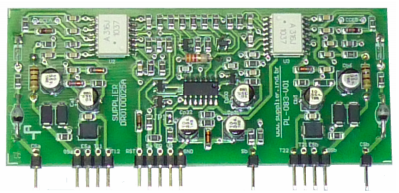
\includegraphics[scale=0.3]{figuras/driver_DRO100D25A.png}
    \caption{\textit{Gate driver} DRO100D25A. Fonte: Supplier}
    \label{fig:driver-DRO100D25A}
    \end{center}
\end{figure}

Ressalta-se que os \textit{gate drivers} possuem dois canais independentes para controle das chaves, isolação óptica, proteção contra curto-circuito através do monitoramento de $V_{ce}$, intertravamento (\textit{interlock}) com configuração de tempo morto e proteção contra subtensão na alimentação do secundário.
A tensão de acionamento dos \textit{drivers} é 15 V, sendo necessário uma interface entre a tensão de saída do microcontrolador de 3,3 V para a entrada de 15 V.

\subsection{Filtro LCL}

Com base nas equações definidas na Seção \ref{filtro-lcl} e com os parâmetros de projeto definidos na Tabela \ref{tab:parametros-inversor}, é possível calcular os parâmetros do filtro LCL a ser utilizado no protótipo.
O Anexo \ref{codigo-python-filtro} apresenta um programa em Python que auxilia nos cálculos dos componentes do filtro LCL baseado nos requisitos de projeto apresentados.

A Tabela \ref{tab:resultados-filtro-lcl} apresenta os resultados obtidos para o filtro LCL.

\begin{table}[h]
	\centering
	\caption{Parâmetros Nominais do Inversor}
	\label{tab:parametros-inversor}

	\begin{tabular}{cc}
		\toprule
		\textbf{Parâmetro} & \textbf{Unidade Equivalente} \\
		\midrule
		Potência Nominal do Inversor & 10 kW \\
		Tensao do Barramento & 680 V \\
		Tensao Nominal CA ($V_n$) & 380 V \\
		Máxima Variação do Fator de Potência ($x$) & 0,063 \\
		Frequência de Chaveamento ($f_{sw}$) & 5000 Hz \\
		Frequência da Rede ($f_n$) & 60 Hz \\
		Ripple de corrente na indutância do lado do conversor ($i_{L-max}$) &  25 \% \\
		Atenuação do ripple de corrente ($\frac{i_{rede}}{i_{ripple}}$) & 10 \% \\
		\bottomrule
	\end{tabular}
\end{table}

\begin{table}[h]
	\centering
	\caption{Resultados para o filtro LCL}
	\label{tab:resultados-filtro-lcl}
	
	\begin{tabular}{cc}
		\toprule
		\textbf{Resultados} & \textbf{Unidade Equivalente} \\
		\midrule
		Indutor do lado do conversor ($L_1$) & 1,5 mH \\
		Indutor do lado da rede ($L_2$) & 1,5 mH \\
		Capacitor ($C_f$) & 11,5 $\mu$F \\
		Resistor de Amortecimento ($R_f$) & 3 $\Omega$ \\
		\bottomrule
	\end{tabular}
\end{table}

\subsection{Conversor \textit{Boost}}

A Tab. \ref{tab:conversor-boost-componentes} mostra os componentes utilizados pelo 
conversor \textit{boost} e seus valores/especificação.

\begin{table}
	\centering
	\caption{Componentes e seus valores utilizados para o conversor \textit{boost}}
	\label{tab:conversor-boost-componentes}
	\begin{tabular}{cc}
		\toprule
		\textbf{Componente} & \textbf{Valor/Especificação} \\
		\midrule
		Capacitor de entrada ($C_1$) & 470 $\mu$F \\
		Capacitor de saída ($C_2$) & 680 $\mu$F \\
		Indutor ($L$)& 2,3 mH \\
		IBGT & G80N60 \\
		\bottomrule
	\end{tabular}

\end{table}

\section{Aquisição e Condicionamento de Sinais}

A etapa de aquisição e condicionamento de sinais destina-se à correta obtenção das tensões e correntes no ponto de acomplamento do inversor com a rede elétrica, e tem como objetivo entregar os parâmetros necessários para a realização do algoritmo de controle implementado no microcontrolador.
Desta forma, é nececessário monitorar três sinais de tensão e três sinais de corrente, e também o valor de tensão no barramento CC.
Os procedimentos realizados nesta etapa são:
\begin{enumerate}
	\item Adaptação e isolação elétrica dos sinais medidos através de níveis de tensão seguros para a etapa de amostragem;
	\item Filtragem dos sinais obtidos de forma a obter os componentes em frequência desejados para o algoritmo de controle;
	\item Ajuste dos níveis de tensão dos sinais obtidos para os limites de tensão impostos pelo ADC do microcontrolador.
\end{enumerate}

O sistema de aquisição e condicionamento de sinais é constituído por:

\begin{itemize}
	\item Transdutores de tensão e corrente;
	\item Filtros \textit{anti-aliasing}, somadores e reguladores de tensão.
\end{itemize}

\subsection{Microcontrolador}

No presente trabalho optou-se pela utilização do modelo TMS320F28335 da Texas Instruments, que pode ser visualizado na Fig. \ref{fig:dsp}.
Este microcontrolador é comumente utilizado em aplicações envolvendo controle industrial de motores, inversores fotovoltaicos e eletrônica de potência \cite{texasinstruments:tms320f28335}.

\begin{figure}[!hbt]
    \begin{center}
    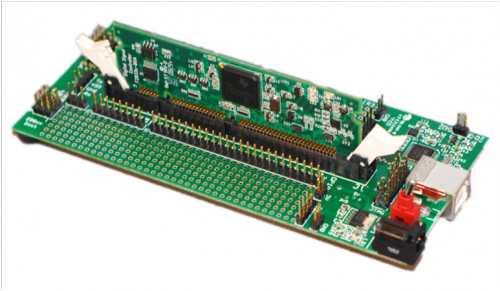
\includegraphics[scale=0.3]{figuras/tms320f28335.png}
    \caption{DSP TMS320F28335}
    \label{fig:dsp}
    \end{center}
\end{figure}

Algumas características interessantes deste microcontrolador são:
\begin{itemize}
    \item Frequência de operação: 150 MHz;
    \item Unidade de ponto flutuante (FPU) em hardware de 32 bits conforme IEEE 754;
    \item Memória RAM: 68 kB;
    \item Memória FLASH: 512 kB;
    \item ADC de 12 bits com 16 canais.
\end{itemize}

\subsection{Transdutores de Tensão e de Corrente}

Para a leitura dos sinais de tensão da rede é utilizado o transdutor de efeito Hall LV-20P mostrado na Fig. \ref{fig:transdutor_tensao}. 

\begin{figure}[!hbt]
	\centering
	\begin{subfigure}[b]{0.4\textwidth}
		\centering
		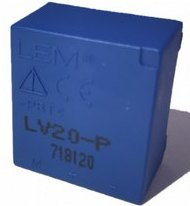
\includegraphics[width=0.5\textwidth]{figuras/Transdutor_Tensao.jpg}
		\caption{Vista frontal do trandutor}
	\end{subfigure}
	\begin{subfigure}[b]{0.4\textwidth}
		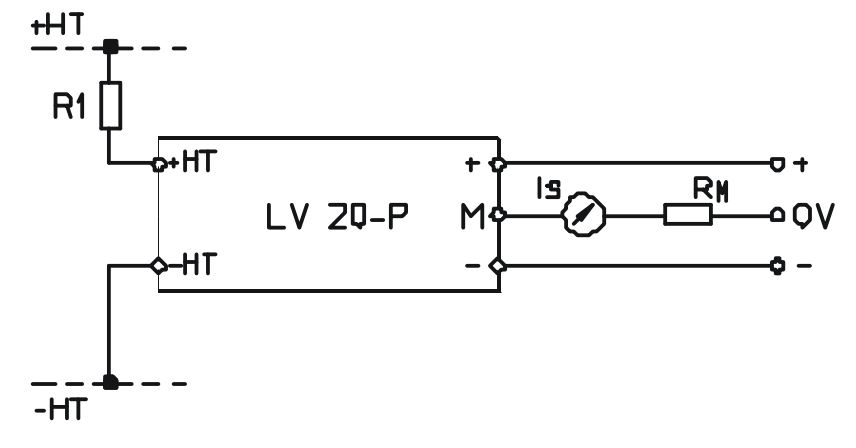
\includegraphics[width=\textwidth]{figuras/Transdutor_Tensao_Circuito.jpg}
		\caption{Circuito do transdutor}
	\end{subfigure}
	\caption{Transdutor de tensão LV-20P}\label{fig:transdutor_tensao}
\end{figure}

Já para a adaptação dos sinais de corrente é utilizado o transdutor de efeito Hall LV-55P mostrado na Fig. \ref{fig:transdutor_corrente}.

\begin{figure}
	\centering
	\begin{subfigure}[b]{0.4\textwidth}
		\centering
		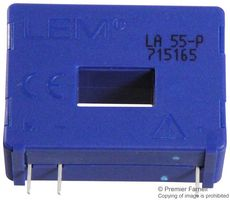
\includegraphics[width=0.5\textwidth]{figuras/Transdutor_Corrente.jpg}
		\caption{Vista frontal do trandutor}
	\end{subfigure}
	\begin{subfigure}[b]{0.4\textwidth}
		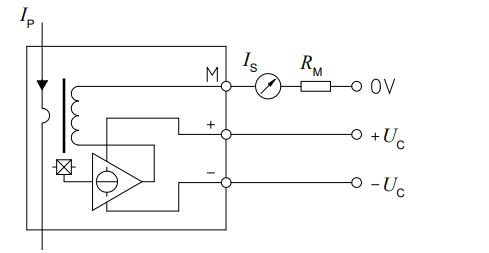
\includegraphics[width=\textwidth]{figuras/Transdutor_Corrente_Circuito.jpg}
		\caption{Circuito do transdutor}
	\end{subfigure}
	\caption{Transdutor de corrente LV-55P}\label{fig:transdutor_corrente}
\end{figure}

\subsection{Filtro \textit{Anti-Aliasing}}

	Uma vez realizada a aquisição dos sinais de interesse através dos transdutores, estes devem estar adequados para que sua manipulação por meio do microcontrolador seja possível.
	Estes sinais podem conter ruídos e transitórios eletromagnéticos inerentes à rede elétrica que são indesejáveis e tendem a provocar o denominado efeito \textit{aliasing}, que causa a sobreposição do espectro e distorções dos sinais analógicos amostrados.
	A obtenção dos sinais relevantes para este trabalho é realizada à uma frequência de amostragem $f_s$ de 10 kHz. O teorema de Nyquist define que para que o sinal analógico de interesse possa ser amostrado corretamente, a frequência $f_{max}$ deste deve ser menor ou igual à metade da frequência de amostragem, conforme a Eq. \ref{eq:freq_sinal} \cite{alanoppenheim2009}.

	\begin{align}
		f_{max} = \frac{f_s}{2}\label{eq:freq_sinal}
	\end{align}

	Com isto, utiliza-se um filtro passa-baixa da topologia \textit{Sallen-Key} de segunda ordem com frequência de corte em 5 kHz e ganho K = 1. A topologia física deste é apresentada na Fig. \ref{fig:filtro-sallen}.
	
	\begin{figure}[!hbt]
			\begin{center}
			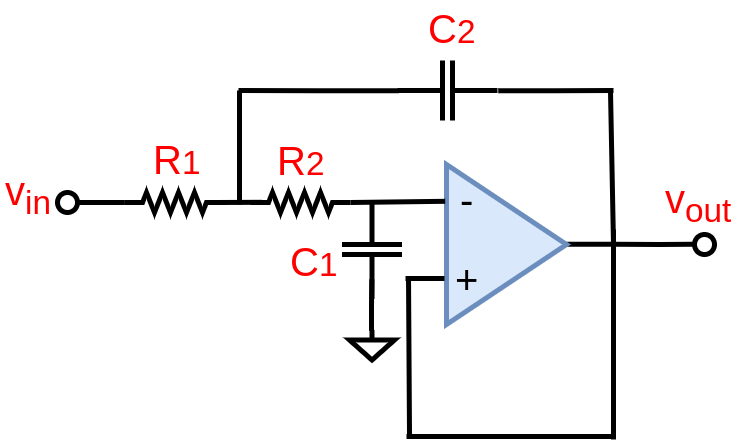
\includegraphics[scale=0.25]{figuras/sallen_key.png}
			\caption{Filtro do tipo \textit{Sallen-Key} de segunda ordem utilizado na placa de condicionamento de sinais}
			\label{fig:filtro-sallen}
			\end{center}
	\end{figure}

%	A frequência de corte $f_c$ deste filtro é dado pela Eq. \ref{eq:freq_corte_butter} e o ganho $K$ é dado pela Eq. \ref{eq:ganho_butter}.
%	
%	\begin{align}
%		f_{c} = \frac{1}{2\pi R_1 C} \label{eq:freq_corte_butter} \\
%		K = -\frac{R_2}{R_1}\label{eq:ganho_butter}
%	\end{align}

\subsection{Circuito Somador}

Um circuito com amplificador operacional na topologia de somador é necessário para que se adicione um nível DC ao sinal proviniente do filtro \textit{anti-aliasing}, de forma que o sinal a ser amostrado reproduza apenas valores positivos compatíveis com os limites de tensão do conversor A/D do microcontrolador. 
A topologia escolhida foi a de \textbf{somador não-inversor}, pois esta não altera os ângulos de fase dos sinais provenientes dos transdutores. A Figura \ref{fig:somador-ninversor} mostra o circuito do somador não inversor. A Eq. \ref{eq:circuito-somador} relaciona a tensão de saída com as tensões de entrada, onde $V_{REF}$ é a tensão de nível CC que é somada ao sinal que vem do filtro anti-aliasing, $V_1$.

\begin{align}
	V_{out} = \left(1+\frac{R_a}{R_b}\right)\left(\frac{V_1/R_1 + V_{REF}/R_2}{1/R_1 + 1/R_2}\right)\label{eq:circuito-somador}
\end{align}

\begin{figure}[!hbt]
	% Center the figure.
	\begin{center}
		% Include the eps file, scale it such that it's width equals the column width. You can also put width=8cm for example...
		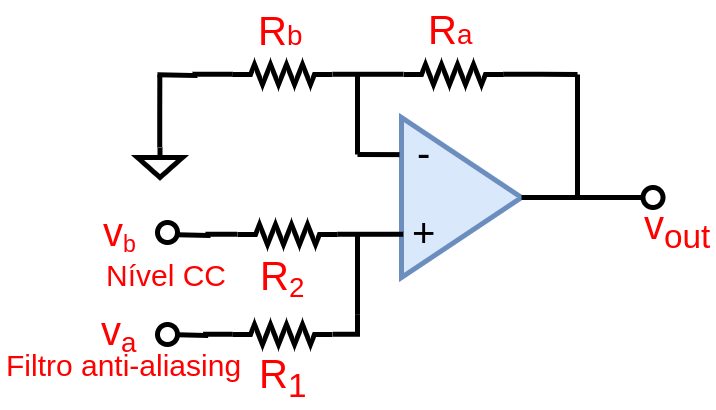
\includegraphics[scale=0.25]{figuras/Somador_Nao-Inversor.png}
		% Create a subtitle for the figure.
		\caption{Circuito somador não-inversor}
		% Define the label of the figure. It's good to use 'fig:title', so you know that the label belongs to a figure.
		\label{fig:somador-ninversor}
	\end{center}
\end{figure}

\subsection{Circuito de fornecimento de tensão CC}

Um outro circuito, anterior ao somador não-inversor, é utilizado para fornecer a tensão CC regulável ao somador.
A Fig. \ref{fig:divisor-tensao} mostra a topologia do circuito. A resistência variável conectada ao amplificador operacional permite o ajuste fino do divisor de tensão.

\begin{figure}[!hbt]
	% Center the figure.
	\begin{center}
		% Include the eps file, scale it such that it's width equals the column width. You can also put width=8cm for example...
		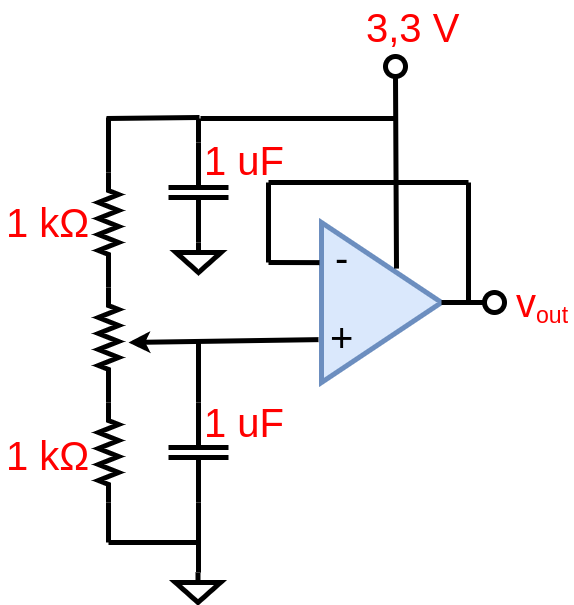
\includegraphics[scale=0.25]{figuras/divisor-tensao.png}
		% Create a subtitle for the figure.
		\caption{Divisor de tensão com resistência variável}
		% Define the label of the figure. It's good to use 'fig:title', so you know that the label belongs to a figure.
		\label{fig:divisor-tensao}
	\end{center}
\end{figure}

\subsection{Circuito Regulador de Tensão}

O circuito de regulação e filtragem de tensão destina-se ao suprimento de tensão aos amplificadores operacionais e transdutores da placa de aquisição. A Fig. \ref{fig:circuito-regulacao} mostra os componentes deste circuito. Este é basicamente composto por \textit{beads} de ferrite e capacitores destinados à minimização de ruídos existentes na tensão de suprimento da placa. A placa de aquisição de sinais é alimentada por uma fonte externa que deve dispor de tensões contínuas de +15 V e -15 V.

\begin{figure}[!hbt]
	% Center the figure.
	\begin{center}
		% Include the eps file, scale it such that it's width equals the column width. You can also put width=8cm for example...
		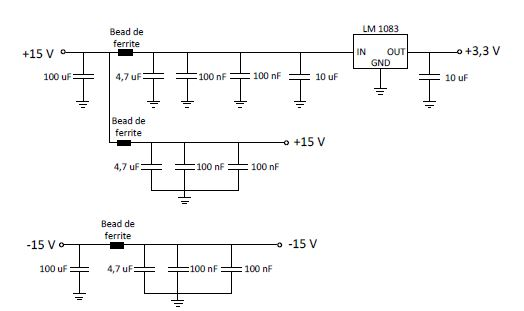
\includegraphics[scale=0.7]{figuras/circuito-regulador.JPG}
		% Create a subtitle for the figure.
		\caption{Circuito para regulação e filtragem de tensão}
		% Define the label of the figure. It's good to use 'fig:title', so you know that the label belongs to a figure.
		\label{fig:circuito-regulacao}
	\end{center}
\end{figure}

\section{Procedimentos para obtenção dos resultados}

\subsection{Procedimentos para os resultados de simulação computacional}

A etapa de simulação computacional teve o objetivo de validar a estrutura física de 
potência utilizada (filtro LCL, inversor trifásico, conversor \textit{boost}) e 
os algoritmos de controle e de sincronização. Para isto, as simulações foram 
realizadas no \textit{software} \textbf{PSIM}, da empresa \textbf{Powersim}, que é 
um simulador voltado mais especificamente para projetos de eletrônica de potência.

As etapas de simulação consistiram em:
\begin{itemize}
	\item Montagem das estrutura física de potência do inversor, filtro, rede elétrica e conversor \textit{boost};
	\item Montagem de blocos com os códigos em C para realização dos algoritmos de controle e de sincronia;
	\item Conexão dos blocos;
	\item Simulação do sistema sem injeção de potência no barramento, ou seja, o inversor atuava como STATCOM;
	\item Simulação do sistema com a injeção de potência constante através do conversor \textit{boost};
	\item Simulação do sistema com a injeção de potência variável através do conversor \textit{boost}.
\end{itemize}

\subsection{Procedimentos para os resultados experimentais}

A etapa experimental visou a montagem física da bancada do inversor trifásico e seus componentes.
Os procedimentos que foram realizados neste trabalho foram:
\begin{itemize}
	\item Montagem do filtro LCL utilizado
	\item Montagem e calibração das placas de condicionamento de sinais
	\item Conexão das placas de condicionamento com o DSP
	\item Calibração do \textit{trimpot} de cada placa de aquisição de sinais para ajuste do nível DC dentro dos limites do conversor A/D
	\item Conexão do DSP com a placa de conversão de pulsos de 3,3 V para 15 V
	\item Conexão da placa de conversão de pulsos com o barramento de controle do inversor trifásico
	\item Ajuste da sequência correta das tensões da rede
	\item Verificação do algoritmo da PLL
	\item Verificação do algoritmo de produção dos pulsos de PWM
	\item Verificação da malha de controle de corrente com inversor isolado
\end{itemize}

Os procedimentos que ainda não foram realizados, mas que estão serão objetivo de etapas futuras
serão:
\begin{itemize}
	\item Teste do inversor na operação como STATCOM
	\item Teste do inversor com a injeção de potência na rede elétrica utilizando o conversor \textit{boost}
\end{itemize}